%        File: prac1.tex
%     Created: Sat Feb 09 01:00  2019 S
% Last Change: Sat Feb 09 01:00  2019 S
%
\documentclass[a4paper, 12pt]{article}
\usepackage[]{amsmath}
\usepackage{amssymb}
\usepackage{float}
\usepackage[]{graphicx}
\usepackage{subfig}
\usepackage{caption}

\title{Control Systems 4A Practical 1 Report}
\author{Ruan de Bruyn, 216054484 \and Quintin Kruger, 216008466}

\begin{document}

\pagenumbering{gobble}
\begin{titlepage}
  \maketitle
\end{titlepage}

\pagenumbering{roman}
\tableofcontents
\newpage
\pagenumbering{arabic}

\section{Transfer Function}
	As a quick summary of the theory given in the practical assignment, the
	equation that governs this system, is given by

	\begin{equation}
	  \frac{d^2}{dt^2} x = -\frac{5g}{7} \sin(\theta)
	  \label{eq:system_complete}
	\end{equation}

	If we make the assumption for this system that the angle $\theta$ is small,
	then we can use small-angle approximation to say that $\sin \theta \approx
	\theta$, and thus \eqref{eq:system_complete} becomes

	\begin{equation}
	  \frac{d^2}{dt^2} x = -\frac{5g}{7} \theta
	  \label{eq:system_simplified}
	\end{equation}

	From here, we can apply a Laplace transform to calculate the transfer function of
	our system, using \eqref{eq:system_simplified}:

	\begin{equation*}
	  \begin{array}{rcl}
		\mathcal{L}\left[ \frac{d^2}{dt^2}x \right] & = & \mathcal{L}\left[ -\frac{5g}{7}\theta \right] \\
		s^2 X(s) & = & -\frac{5g}{7}\Theta(s) \\
		\frac{X(s)}{\Theta(s)}  & = & -\frac{5g}{7s^2} \\
	  \end{array}
	  \label{eq:transfer_function}
	\end{equation*}
	
	Taking the constant $g = 9.8 \, m \cdot s^{-2}$, this leaves us with a final transfer function of

	\begin{equation}
	  T(s) = -\frac{5g}{7s^2} = -\frac{7}{s^2}
	  \label{eq:tf_final}
	\end{equation}

% endsection Transfer Function

\section{Implementation and Analysis}
	The Octave code that was used to design the PID controller in the rest of
	this report is given below\\\\\noindent
\texttt{function plotsys(Kp, Ki, Kd)\\\noindent
  ts = - 5 * 9.8 / (7 * tf('s'));\\\noindent
  sys = feedback(ts * pid(Kp, Ki, Kd))\\\noindent
  step(sys);\\\noindent
endfunction}\\\noindent

This function simply obtains the transfer function obtained in
\eqref{eq:tf_final}, finds the equivalent function of the plant and controller
with the specified constants in a negative feedback loop, and then graphs the
output response. The design strategy of the PID controller for our system is to
have a fairly quick rise time, but also with very little overshoot. A quick
rise time is necessary, because if our system is too slow to react, the ball
may fall off of one of the ends of the beam. Overshoot should be kept as low as
possible as well, because a large overshoot could very well result in the ball
falling off the beam too, especially if the commanding signal desires the
location of the ball to be near one of the edges of the beam.

From theory, we would hypothesize that we should have a large $K_p$ and $K_d$,
as a large $K_p$ would result in a quick rise time and a large $K_d$ would
prevent large amounts of overshoot. $K_i$, then, should be the variable to keep
small in relation to $K_p$ and $K_d$, as $K_i$ contributes to a quick rise
time, but also to overshoot. With this in mind, we choose our variables as
follows:

\begin{equation}
  \begin{array}{rcl}
	K_p & = & 70 \\
	K_i & = & 18 \\
	K_d & = & 40
  \end{array}
  \label{eq:pid_constants}
\end{equation}

The response given by this system of constants is

\begin{figure}[H]
	\centering
	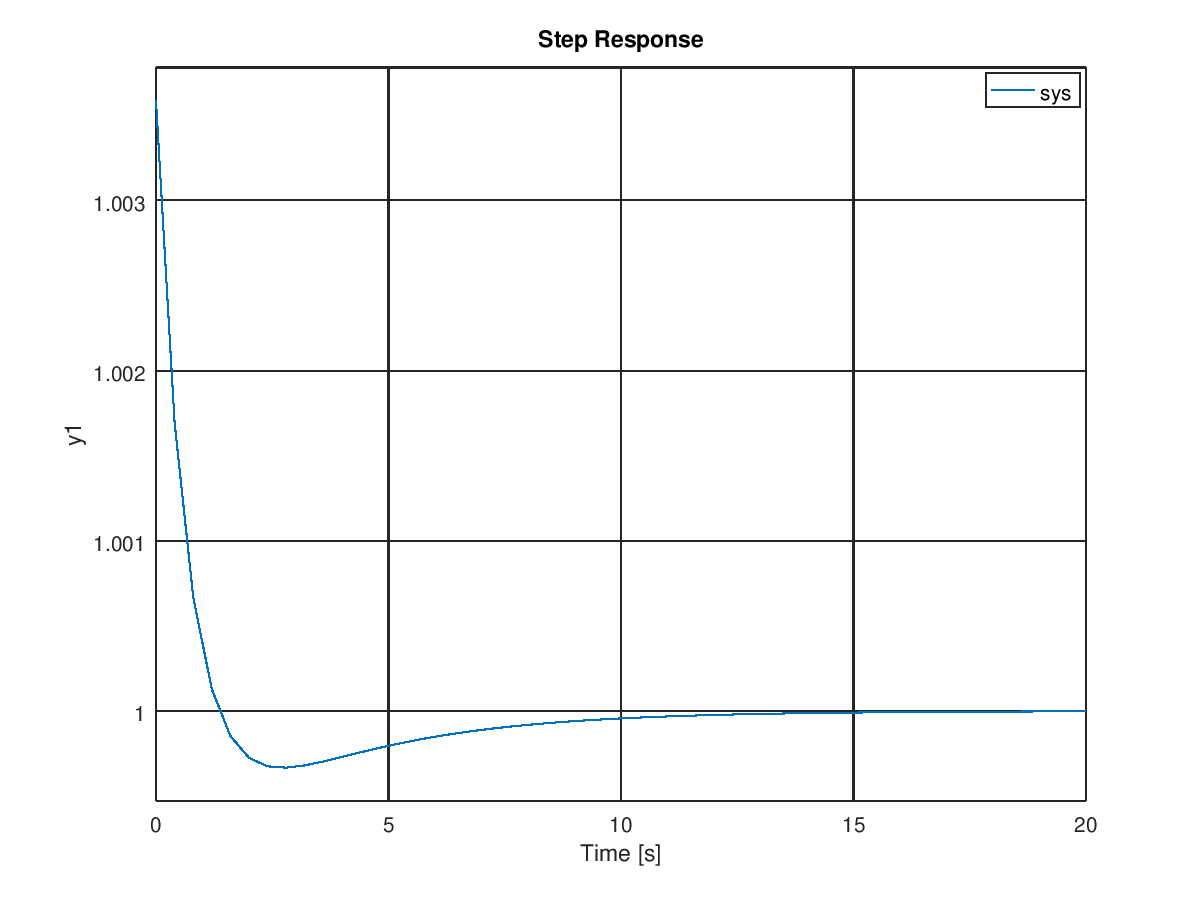
\includegraphics[width=\textwidth]{response.png}
	\caption{System response with constants chosen in \eqref{eq:pid_constants}}
	\label{fig:response}
\end{figure}

If we decide to let the rise time for this system be defined as the time it
takes the response to reach 0.1\% of its final value, then the rise time $t_r
= 0.67s$. The overshoot is 0.9997, which means that $\%OS = 0.03$. Finally, if
we take the settling time to be the time it takes the transfer function to
reach 0.0001 of its final value, then we have $t_s = 7.33s$. The final values
are then summarised below as

\begin{equation}
  \begin{array}{rcl}
    t_r & = & 0.67 \\
    t_s & = & 7.33 \\
    \%OS & = & 0.03 \\
  \end{array}
  \label{eq:finalstats}
\end{equation}

% endsecion Implementation and Analysis
\section{Discussion} % (fold)
\label{sec:discussion}
The controller is used to achieve a desired output. 3 classes of controllers
were used in conjunction with one another to arrive at the final step response
as illustrated by Figure \ref{fig:response}

As a consideration of the PID controller established in this experiment, we
first look at the effect of a proportional controller. By using an integrator
system defined by the transfer function $H = \frac{1}{s}$ we plot the step
response with its associated pole zero plot to show the stability.

\begin{figure}[H]
	\centering
	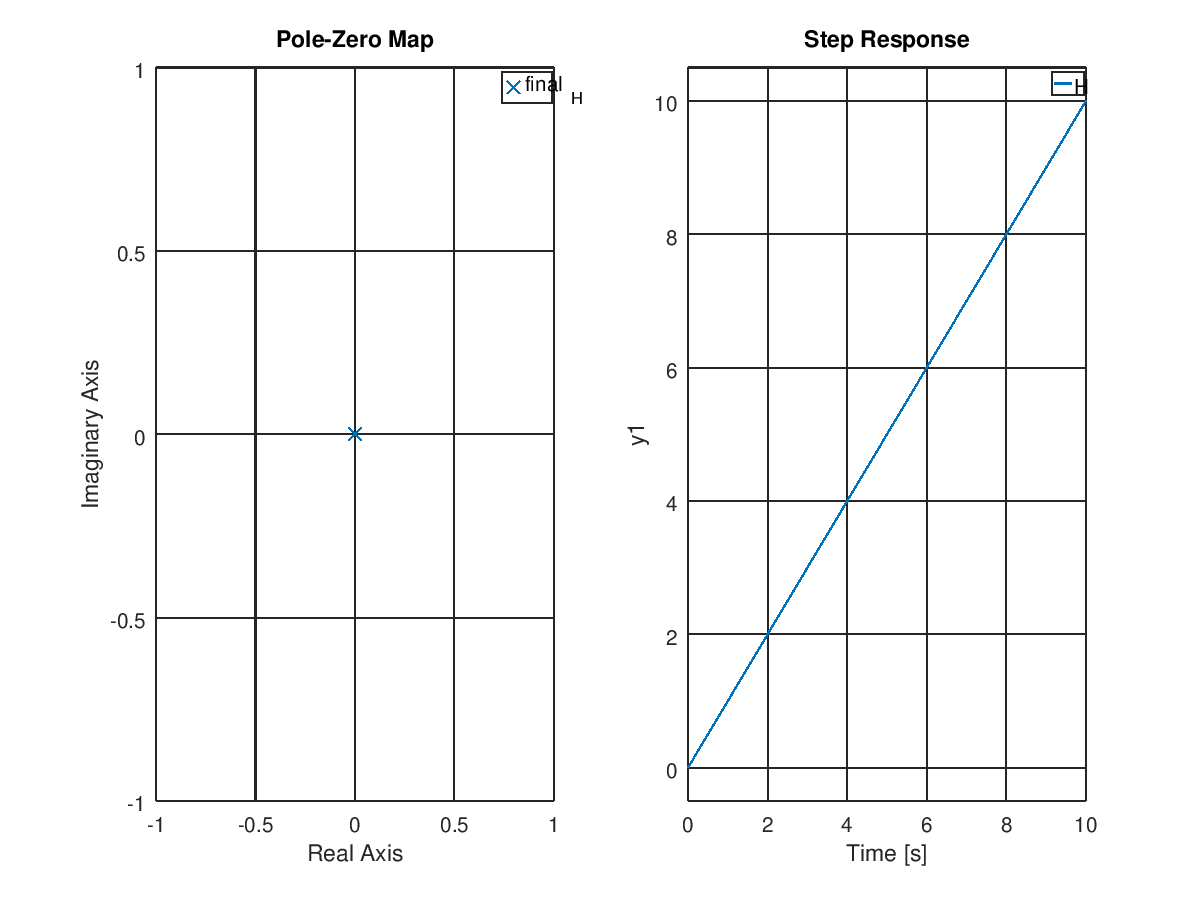
\includegraphics[width=\textwidth]{integrator_system.png}
	\caption{Step response of an integrator system}
	\label{fig:integrator_system}
\end{figure}

The desired response of this system is to be fed an input, to achieve this
input and remain at the desired input value for the duration of another
successive input. We first used a proportional controller to achieve this (the
proportion was chosen to be $K_p = 1$ for purposes of illustration). The
response with the addition of the controller as described is shown below.

\begin{figure}[H]
	\centering
	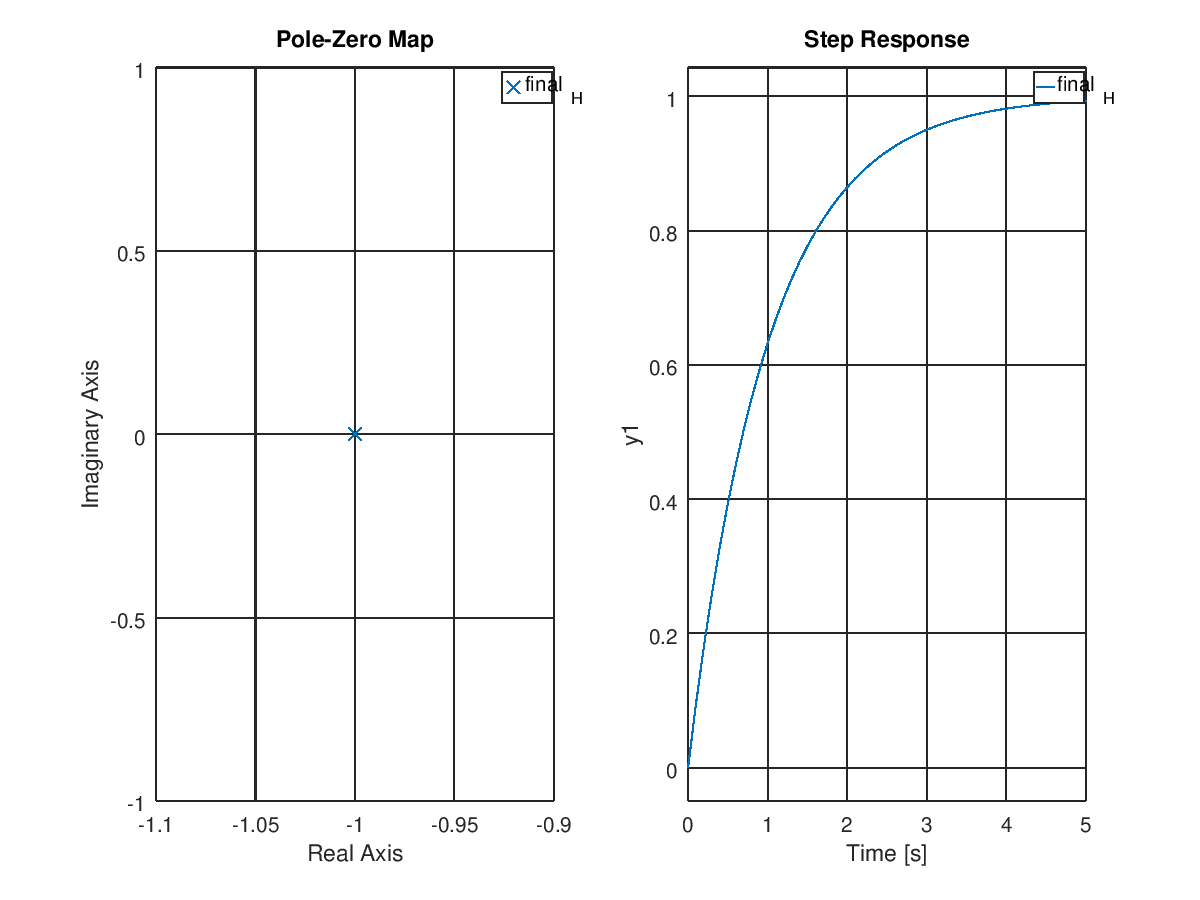
\includegraphics[width=\textwidth]{integrator_system_proportional_controller.png}
	\caption{Integrator system with the addition of a proportional controller}
	\label{fig:integrator_system_proportional_controller}
\end{figure}

The figure shows a system that reaches a steady state value, which is the
desired response but with a steady state error as can be seen from Figure
\ref{fig:integrator_system_proportional_controller}. To get rid of the steady
state error we introduce the PI controller or the proportional integral
controller

\begin{figure}[H]
	\centering
	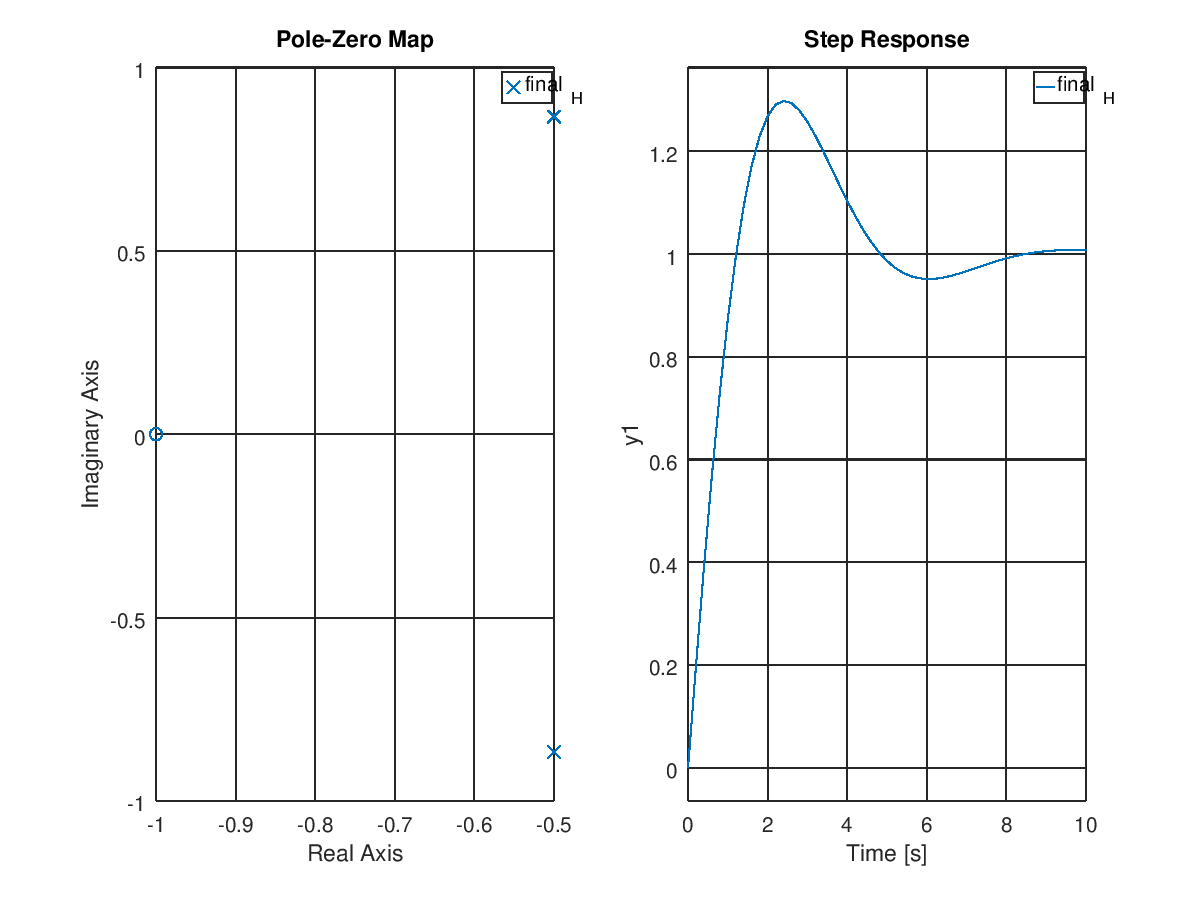
\includegraphics[width=\textwidth]{integrator_system_proportional_integral_controller.png}
	\caption{Integrator system with the addition of a integral proportional controller}
	\label{fig:integrator_system_proportional_integral_controller}
\end{figure}

Notice that the steady state error has been rectified but a transient response
has now been introduced. To rectify this a proportional derivative too has to
be added in addition to the 2 previously discussed controller. The settling
time has increased from a settling time of $5$ seconds to a settling time of
$10$ seconds and the rise time went from $2.5$ seconds to $1$ seconds

\begin{figure}[H]
	\centering
	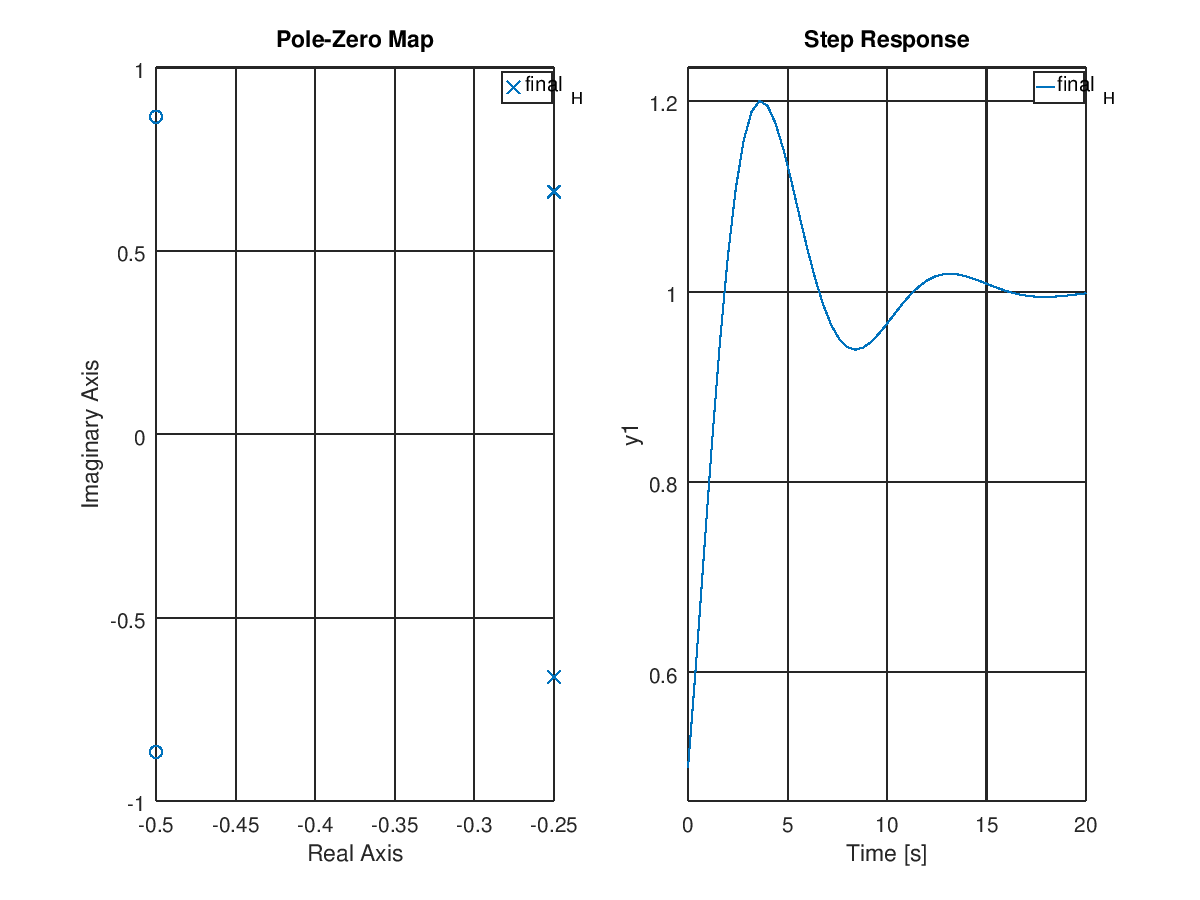
\includegraphics[width=\textwidth]{integrator_system_proportional_integral_derivative_controller.png}
	\caption{Application of the PID controller to an integrator system}
	\label{fig:integrator_system_proportional_integral_derivative_controller}
\end{figure}

Notice the reduction in the percent overshoot from $1.3$ to $1.2$ and still
another increase in the settling time from $10$ seconds to $20$ seconds. The
rise time increased from $1$ second to $2.5$ seconds.

\par

In summary, we can see that the proportional controller allows the system to
reach a steady state value and decreases the settling time. The proportional
integral controller rids the system of steady state error and decreases the
rise time and the derivative controller decreases the percent overshoot of the
system.

Thus, the use of the PID controller results in the desired system with reference
to the improvement with the rise time, settling time and steady state error as
discussed previously.

By increasing the various proportionalities $K_p, K_i$ and $K_d$ the optimal
system was obtained by using trial and error and the pole zero plot illustrated
by each figure from Figure \ref{fig:integrator_system} through Figure
\ref{fig:integrator_system_proportional_integral_derivative_controller} to
ensure a stable system for the varies constants.

% section discussion (end)

\end{document}
